\documentclass[10pt,a4paper]{article}
\usepackage[utf8]{inputenc}
\usepackage{amsmath}
\usepackage{amsfonts}
\usepackage{graphicx}
\usepackage{amssymb}
\usepackage{hyperref}
\usepackage[left=2cm,right=2cm,top=2cm,bottom=2cm]{geometry}
\title{Théorie des graphes}
\date{}
\renewcommand{\contentsname}{Sommaire}
\usepackage{setspace}
\onehalfspacing
\setlength{\parindent}{0pt}

\begin{document}

\section*{Supervised learning: linear regression}

\subsection*{Introduction}

En régression, nous cherchons à modéliser la relation entre des \textbf{caractéristiques} $\mathbf{x}_{i} \in \mathbb{R}^{d}$ et une quantité continue $y_{i} \in \mathbb{R}$ appelée \textbf{réponse}. Les données sont représentées par un ensemble $\mathcal{D}=\left\{\left(\mathbf{x}_{1}, y_{1}\right),\left(\mathbf{x}_{2}, y_{2}\right), \ldots,\left(\mathbf{x}_{N}, y_{N}\right)\right\}$.

L'objectif est d'apprendre une fonction de régression $r: \mathbb{R}^d \to \mathbb{R}$ telle que $r(\mathbf{x}) = \mathbb{E}(y|\mathbf{x})$. Cette fonction permet de prédire la valeur de $y$ pour de nouvelles valeurs de $\mathbf{x}$.

\subsection*{Simple Linear Regression}

\subsubsection*{Modèle}

La régression linéaire simple suppose que $r(x)$ est linéaire :

$$
r(x) = \beta_{0} + \beta_{1} x
$$

où $\beta_{0}$ est l'\textbf{ordonnée à l'origine} (intercept) et $\beta_{1}$ est la \textbf{pente} (slope).

Le modèle de régression linéaire simple est donné par :

$$
y_{i} = r(x_{i}) + \epsilon_{i} = \beta_{0} + \beta_{1} x_{i} + \epsilon_{i}, \quad \epsilon_{i} \sim \mathcal{N}(0, \sigma^{2})
$$

où $x_{i} \in \mathbb{R}$ et $\operatorname{Var}(\epsilon_{i} | x_{i}) = \sigma^{2}$ (homogénéité des variances).

\subsubsection*{Estimation par les moindres carrés}

Les estimateurs des moindres carrés minimisent la somme des carrés des résidus (RSS) :

$$
\text{RSS} = \sum_{i=1}^{N} \hat{\epsilon}_i^2, \quad \text{où} \quad \hat{\epsilon}_i = y_i - \hat{y}_i
$$

La fonction objectif est :

$$
\mathcal{L}(\beta_0, \beta_1) = \sum_{i=1}^{N} (y_i - \beta_1 x_i - \beta_0)^2
$$

Les estimateurs $\hat{\beta}_0$ et $\hat{\beta}_1$ sont obtenus en minimisant $\mathcal{L}(\beta_0, \beta_1)$ :

$$
\hat{\beta}_0, \hat{\beta}_1 = \underset{\beta_0, \beta_1}{\arg \min} \mathcal{L}(\beta_0, \beta_1)
$$

\subsubsection*{Formules des estimateurs}

Les formules pour les estimateurs des moindres carrés sont les suivantes:refs[6-5] :

$$
\bar{x} = \frac{1}{N} \sum_{i=1}^{N} x_{i}, \quad \bar{y} = \frac{1}{N} \sum_{i=1}^{N} y_{i}, \quad \hat{\sigma}^{2} = \frac{1}{N} \sum_{i=1}^{N} \hat{\epsilon}_{i}^{2}
$$

$$
\hat{\beta}_{1} = \frac{\sum_{i=1}^{N}(y_{i}-\bar{y})(x_{i}-\bar{x})}{\sum_{i=1}^{N}(x_{i}-\bar{x})^{2}}, \quad \hat{\beta}_{0} = \bar{y} - \hat{\beta}_{1} \bar{x}
$$

\subsubsection*{Interprétation géométrique}

La méthode des moindres carrés peut être interprétée géométriquement comme la recherche de la ligne qui minimise la somme des carrés des distances verticales entre les points de données et la ligne de régression. Cette ligne est la projection orthogonale des points de données sur le sous-espace engendré par la droite de régression:refs[8-12,13].

% Insérer ici une image montrant la ligne de régression et les résidus.


\subsubsection*{Propriétés des estimateurs}

Sous l'hypothèse de normalité des erreurs, l'estimateur des moindres carrés est également l'estimateur du maximum de vraisemblance. Les propriétés asymptotiques des estimateurs sont les suivantes:refs[10-5] :

- \textbf{Convergence} : $\hat{\beta}_{0} \xrightarrow{P} \beta_{0}$ et $\hat{\beta}_{1} \xrightarrow{P} \beta_{1}$.

- \textbf{Normalité asymptotique} :

$$
\frac{\hat{\beta}_{0}-\beta_{0}}{\hat{se}(\hat{\beta}_{0})} \xrightarrow{D} \mathcal{N}(0,1) \quad \text{et} \quad \frac{\hat{\beta}_{1}-\beta_{1}}{\hat{se}(\hat{\beta}_{1})} \xrightarrow{D} \mathcal{N}(0,1)
$$

où

$$
\hat{se}(\hat{\beta}_{0}) = \frac{\hat{\sigma} \sqrt{\sum_{i=1}^{N} x_{i}^{2}}}{\sqrt{N} \sum_{i=1}^{N}(x_{i}-\bar{x})^{2}}, \quad \hat{se}(\hat{\beta}_{1}) = \frac{\hat{\sigma}}{\sum_{i=1}^{N}(x_{i}-\bar{x})^{2}}
$$

\subsubsection*{Exemple}

Supposons que la vraie fonction de régression soit $r(x) = 5x + 10$. Après estimation, on pourrait obtenir une fonction estimée $\hat{r}(x) = 3.88x + 10.65$, c'est-à-dire $\hat{\beta}_0 = 10.65$ et $\hat{\beta}_1 = 3.88$.

% Insérer ici un graphique montrant la vraie fonction et la fonction estimée.
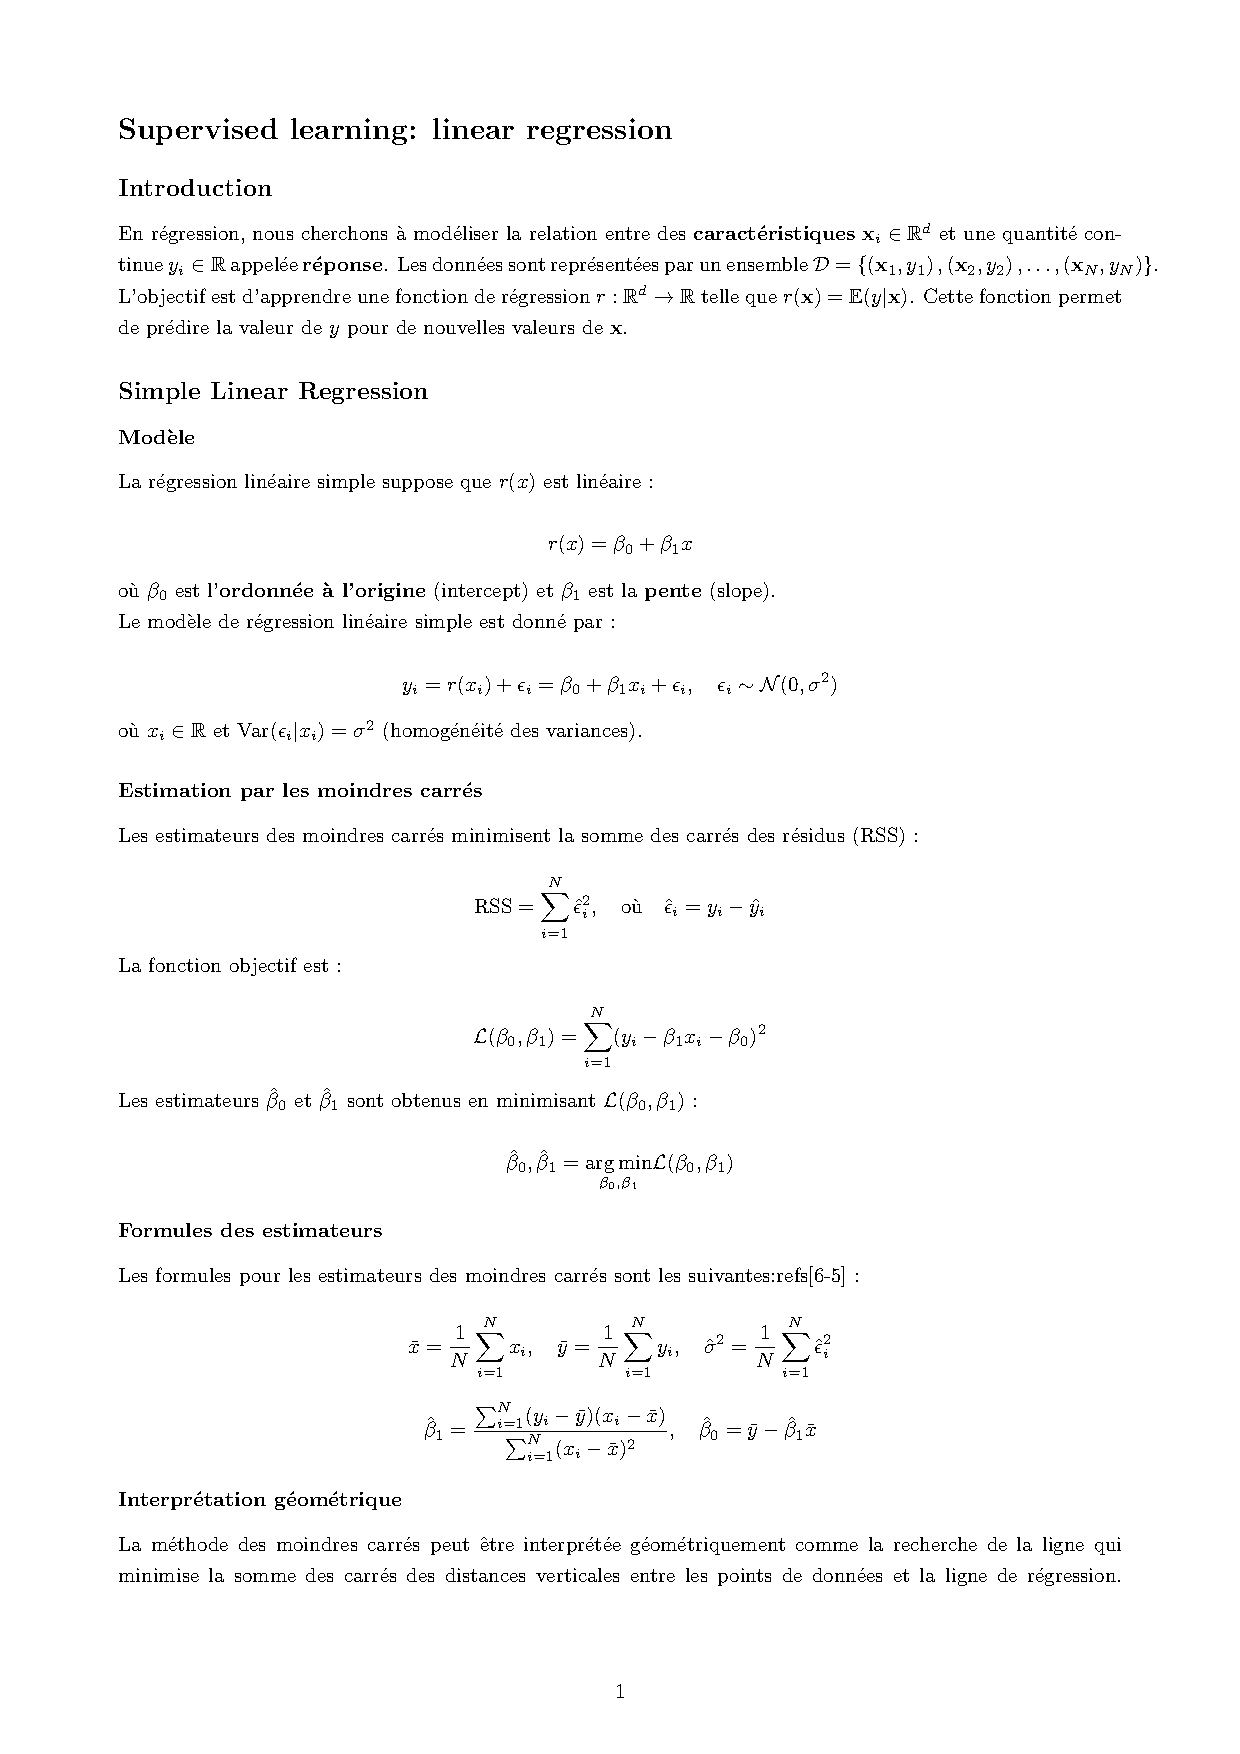
\includegraphics[width = 0.5 \textwidth]{regression.png}

\subsection*{Conclusion}

La régression linéaire simple est une méthode puissante pour modéliser la relation entre une variable explicative et une variable réponse. Les estimateurs des moindres carrés permettent d'obtenir une solution optimale sous des hypothèses de normalité et d'homogénéité des variances. La compréhension de l'interprétation géométrique et des propriétés asymptotiques est essentielle pour une utilisation efficace de cette méthode.

\subsection*{Multiple Regression}

\subsubsection*{Introduction}

Dans le cas où $x_i \in \mathbb{R}^d$, nous avons une régression multiple. Ce modèle peut être généralisé pour modéliser des fonctions de régression non linéaires par expansion de fonctions de base.

Le modèle multidimensionnel est donné par :

$$
y_{i} = \boldsymbol{\beta}^{T} \mathbf{x}_{i} + \epsilon_{i} = \sum_{j=0}^{d} \beta_{j} x_{ij} + \epsilon_{i}
$$

En notation matricielle, cela s'écrit :

$$
\mathbf{y} = \mathbf{X} \boldsymbol{\beta} + \boldsymbol{\epsilon}
$$

où

$$
\mathbf{y} = \begin{bmatrix} y_{1} \\ y_{2} \\ \vdots \\ y_{N} \end{bmatrix}, \quad
\mathbf{X} = \begin{bmatrix}
1 & x_{1,1} & x_{1,2} & \ldots & x_{1,d} \\
1 & x_{2,1} & x_{2,2} & \ldots & x_{2,d} \\
\vdots & \vdots & \vdots & \ddots & \vdots \\
1 & x_{N,1} & x_{N,2} & \ldots & x_{N,d}
\end{bmatrix}, \quad
\boldsymbol{\beta} = \begin{bmatrix} \beta_{0} \\ \beta_{1} \\ \vdots \\ \beta_{d} \end{bmatrix}, \quad
\boldsymbol{\epsilon} = \begin{bmatrix} \epsilon_{1} \\ \epsilon_{2} \\ \vdots \\ \epsilon_{N} \end{bmatrix}
$$

\subsubsection*{Problème d'optimisation}

La fonction objectif pour la régression multiple est :

$$
\mathcal{L}(\boldsymbol{\beta}) = \frac{1}{2}\|\mathbf{y} - \mathbf{X} \boldsymbol{\beta}\|_{2}^{2} = \frac{1}{2} \sum_{i=1}^{N}\left(y_{i} - \left(\beta_{0} + \sum_{j=1}^{d} \beta_{j} x_{ij}\right)\right)^{2}
$$

Cette fonction est convexe, ce qui garantit l'existence d'un minimum global unique:refs[1-9].

\subsubsection*{Solution analytique}

La solution optimale pour $\boldsymbol{\beta}$ est donnée par :

$$
\hat{\boldsymbol{\beta}} = \underset{\boldsymbol{\beta}}{\arg \min} \, \mathcal{L}(\boldsymbol{\beta})
$$

Si la matrice $\mathbf{X}^{T} \mathbf{X}$ est inversible, la solution est :

$$
\hat{\boldsymbol{\beta}} = (\mathbf{X}^{T} \mathbf{X})^{-1} \mathbf{X}^{T} \mathbf{y} = \mathbf{X}^{\dagger} \mathbf{y}
$$

où $\mathbf{X}^{\dagger}$ est la pseudo-inverse de Moore-Penrose de $\mathbf{X}$:refs[3-9].

\subsubsection*{Interprétation géométrique}

Les valeurs ajustées aux entrées d'entraînement sont données par :

$$
\hat{\mathbf{y}} = \mathbf{X} \hat{\boldsymbol{\beta}} = \mathbf{X} \mathbf{X}^{\dagger} \mathbf{y} = \mathbf{P} \mathbf{y}
$$

où $\mathbf{P}$ est la matrice de projection orthogonale de $\mathbf{y}$ sur le sous-espace vectoriel engendré par les colonnes de $\mathbf{X}$. Cette matrice satisfait $\mathbf{P}^2 = \mathbf{P}$ et $\mathbf{P}^T = \mathbf{P}$:refs[5-17].

% Insérer ici une image montrant la projection orthogonale de y sur le sous-espace engendré par les colonnes de X.
\includegraphics[scale=0.5]{projection.png}

\subsubsection*{Propriétés des estimateurs}

L'estimateur des moindres carrés $\hat{\boldsymbol{\beta}}$ est sans biais ($\mathbb{E}[\hat{\boldsymbol{\beta}}] = \boldsymbol{\beta}$) et sa variance est :

$$
\operatorname{Var}(\hat{\boldsymbol{\beta}}) = \sigma^{2}(\mathbf{X}^{T} \mathbf{X})^{-1}
$$

L'estimateur est asymptotiquement efficace, c'est-à-dire qu'il atteint la borne de Cramér-Rao pour de grands $N$:refs[7-9].

\subsubsection*{Interprétation des coefficients}

Les coefficients $\hat{\beta}_j$ indiquent l'importance de chaque caractéristique $x_j$ dans le modèle. Plus un coefficient est proche de zéro, moins la caractéristique correspondante est pertinente. On peut également construire des intervalles de confiance pour chaque coefficient en utilisant leur distribution asymptotique gaussienne:refs[9-9].

\subsubsection*{Expansion de fonctions de base}

Pour modéliser des relations non linéaires, on peut remplacer $\mathbf{x}$ par une fonction $\phi(\mathbf{x}): \mathbb{R}^{d} \rightarrow \mathbb{R}^{d^{*}}$. Le nouveau modèle devient :

$$
y_{i} = \boldsymbol{\beta}^{T} \phi(\mathbf{x}_{i}) + \epsilon_{i} = \sum_{j=0}^{d^{*}} \beta_{j} \phi_{j}(\mathbf{x}_{i}) + \epsilon_{i}
$$

En notation matricielle :

$$
\mathbf{y} = \boldsymbol{\Phi} \boldsymbol{\beta} + \boldsymbol{\epsilon}
$$

où $\boldsymbol{\Phi}$ est la matrice de conception après transformation des données. Cette approche est appelée \textbf{expansion de fonctions de base}:refs[11-20,27].

\subsubsection*{Exemples de fonctions de base}

- \textbf{Basis polynomiale} : $\phi(\mathbf{x}) = [1, x, x^2, \ldots, x^{d^{*}}]$.

- \textbf{Basis gaussienne} : $\phi_j(\mathbf{x}) = \exp\left(-\frac{\|\mathbf{x} - \boldsymbol{\mu}_j\|^2}{2s^2}\right)$, où $\boldsymbol{\mu}_j$ sont les centres et $s$ est l'écart-type:refs[13-23].

% Insérer ici un graphique montrant un exemple d'expansion de fonctions de base (polynomiale ou gaussienne).
\includegraphics[scale=0.3]{polynomiale}

\includegraphics[scale=0.3]{gaussienne}

\subsubsection*{Conclusion}

La régression multiple permet de modéliser des relations complexes entre plusieurs variables explicatives et une variable réponse. L'expansion de fonctions de base offre une flexibilité supplémentaire pour capturer des relations non linéaires, tout en conservant la convexité du problème d'optimisation.

\subsection*{Regularized Linear Regression}

\subsubsection*{Introduction}

La régularisation permet de contrôler le degré de lissage de la solution et de traiter le surapprentissage. Elle consiste à ajouter un terme de régularisation à la fonction objectif du problème d'optimisation. Par exemple, la fonction objectif régularisée peut s'écrire :

$$
\mathcal{L}_{\text{reg}}(\boldsymbol{\beta}) = \frac{1}{2}\|\mathbf{y} - \mathbf{X} \boldsymbol{\beta}\|_{2}^{2} + \alpha \|\boldsymbol{\beta}\|_{q}^{q}
$$

où $\alpha$ est le paramètre de régularisation et $\|\boldsymbol{\beta}\|_{q} = \left(\sum_{i=1}^{d} |\beta_i|^{q}\right)^{1/q}$:refs[1-30].

\subsubsection*{Régularisation $\ell_2$ : Ridge Regression}

La régularisation $\ell_2$ (ou Ridge Regression) utilise $q=2$ :

$$
\mathcal{L}_{\text{ridge}}(\boldsymbol{\beta}) = \frac{1}{2}\|\mathbf{y} - \mathbf{X} \boldsymbol{\beta}\|_{2}^{2} + \frac{\alpha}{2} \|\boldsymbol{\beta}\|_{2}^{2}
$$

La solution explicite pour $\hat{\boldsymbol{\beta}}$ est :

$$
\hat{\boldsymbol{\beta}} = (\mathbf{X}^{T} \mathbf{X} + \alpha \mathbf{I})^{-1} \mathbf{X}^{T} \mathbf{y}
$$

La régularisation Ridge réduit la magnitude des coefficients, mais ne les annule pas complètement:refs[3-30,33].

\subsubsection*{Régularisation $\ell_1$ : Lasso Regression}

La régularisation $\ell_1$ (ou Lasso Regression) utilise $q=1$ :

$$
\mathcal{L}_{\text{lasso}}(\boldsymbol{\beta}) = \frac{1}{2}\|\mathbf{y} - \mathbf{X} \boldsymbol{\beta}\|_{2}^{2} + \alpha \|\boldsymbol{\beta}\|_{1}
$$

Contrairement à la Ridge, la Lasso peut annuler certains coefficients, ce qui permet une sélection automatique des caractéristiques:refs[5-30,34].

\subsubsection*{Interprétation géométrique}

- **Ridge** : La contrainte est une boule $\ell_2$, ce qui conduit à une réduction uniforme des coefficients.

- **Lasso** : La contrainte est un diamant $\ell_1$, ce qui favorise des solutions clairsemées (certains coefficients sont exactement nuls):refs[7-31].

% Insérer ici une image montrant les contraintes géométriques pour Ridge et Lasso.
\includegraphics[scale=0.3]{ridge lasso}

\subsubsection*{Exemple}

Supposons que les coefficients estimés sans régularisation soient :

$$
\hat{\beta} = [7.70, 660.66, -10182.54, -443729.74, 18829790.68, \ldots]
$$

Avec la régularisation $\ell_2$ (Ridge), les coefficients deviennent :

$$
\hat{\beta}_{\text{ridge}} = [12.76, 40.53, -184.92, 93.17, 145.81, \ldots]
$$

Avec la régularisation $\ell_1$ (Lasso), les coefficients deviennent :

$$
\hat{\beta}_{\text{lasso}} = [0, 0.27, -65.86, 56.86, 55.20, \ldots]
$$

On observe que la régularisation réduit la magnitude des coefficients, et que la Lasso peut annuler certains d'entre eux:refs[9-30].

\subsubsection*{Perspective bayésienne}

La régularisation peut être interprétée comme un estimateur du maximum a posteriori (MAP). Si la distribution a priori $p(\boldsymbol{\beta})$ est gaussienne, on obtient la régularisation Ridge. Si elle est laplacienne, on obtient la régularisation Lasso:refs[11-34].

\subsubsection*{Conclusion}

La régularisation est un outil puissant pour éviter le surapprentissage et améliorer la généralisation du modèle. Ridge et Lasso sont deux méthodes courantes, chacune ayant ses propres avantages : Ridge réduit uniformément les coefficients, tandis que Lasso permet une sélection de caractéristiques.

\subsection*{Bias-variance tradeoff}

\subsubsection*{Introduction}

Le compromis biais-variance est un concept fondamental en apprentissage supervisé. Il décrit la relation entre la complexité d'un modèle, la précision de ses prédictions, et sa capacité à généraliser à de nouvelles données:refs[1-40].

L'erreur quadratique moyenne attendue sur une nouvelle donnée $\mathbf{x}$ peut être décomposée comme suit :

$$
\mathbb{E}\left[(y - \hat{r}(\mathbf{x}; \mathcal{D}))^{2}\right] = \text{Bias}(\hat{r}(\mathbf{x}; \mathcal{D}))^{2} + \text{Var}(\hat{r}(\mathbf{x}; \mathcal{D})) + \sigma^{2}
$$

où :
- $\text{Bias}(\hat{r}(\mathbf{x}; \mathcal{D}))^{2} = (\mathbb{E}[\hat{r}(\mathbf{x}; \mathcal{D})] - r(\mathbf{x}))^2$,
- $\text{Var}(\hat{r}(\mathbf{x}; \mathcal{D})) = \mathbb{E}[(\hat{r}(\mathbf{x}; \mathcal{D}) - \mathbb{E}[\hat{r}(\mathbf{x}; \mathcal{D})])^2]$,
- $\sigma^2$ est la variance du bruit inhérent aux données:refs[3-40].

\subsubsection*{Démonstration mathématique}

En développant l'erreur quadratique moyenne, on obtient :

$$
\mathbb{E}\left[(y - \hat{r}(\mathbf{x}; \mathcal{D}))^{2}\right] = \mathbb{E}\left[y^{2} + \hat{r}(\mathbf{x}; \mathcal{D})^{2} - 2y\hat{r}(\mathbf{x}; \mathcal{D})\right]
$$

En utilisant les propriétés de l'espérance et de la variance, on peut montrer que :

$$
\mathbb{E}\left[(y - \hat{r}(\mathbf{x}; \mathcal{D}))^{2}\right] = \sigma^{2} + \text{Var}(\hat{r}(\mathbf{x}; \mathcal{D})) + (\text{Bias}(\hat{r}(\mathbf{x}; \mathcal{D})))^{2}
$$

Cette décomposition montre que l'erreur totale est la somme du biais au carré, de la variance, et de la variance du bruit:refs[5-40,47].

\subsubsection*{Cas extrêmes}

\paragraph{Underfitting}

Si le modèle est trop simple (par exemple, une constante $\hat{r}(\mathbf{x}; \mathcal{D}) = c$), alors :

$$
\text{GE} = (c - r(\mathbf{x}))^2 + 0 + \sigma^2
$$

Le biais est élevé car le modèle ne capture pas la complexité des données, mais la variance est nulle:refs[7-40].

\paragraph{Overfitting}

Si le modèle est trop complexe (par exemple, $\hat{r}(\mathbf{x}; \mathcal{D}) = r(\mathbf{x}) + \gamma(\mathcal{D})$, où $\gamma(\mathcal{D})$ est un bruit), alors :

$$
\text{GE} = 0 + \text{Var}(\gamma(\mathcal{D})) + \sigma^2
$$

La variance est élevée car le modèle capture le bruit dans les données d'entraînement:refs[9-40].

\subsubsection*{Compromis biais-variance}

En pratique, il y a toujours un compromis entre le biais et la variance :

- Réduire le biais augmente généralement la variance.

- Réduire la variance augmente généralement le biais.

La régularisation permet de trouver un équilibre en augmentant légèrement le biais pour réduire significativement la variance, ce qui améliore la généralisation du modèle:refs[11-40].

\subsubsection*{Sélection de modèle}

Pour choisir un bon modèle, on peut utiliser des critères comme :

- \textbf{Mean Squared Error (MSE)} : $\text{MSE} = \frac{1}{N} \sum_{i=1}^{N}(y_i - \hat{y}_i)^2$,

- \textbf{Coefficient de détermination ($R^2$)} : $R^2 = 1 - \frac{\text{RSS}}{\sum_{i=1}^{N}(y_i - \bar{y})^2}$,

- \textbf{Akaike Information Criterion (AIC)} : $\text{AIC} = \ell(\hat{\beta}) - \text{\# features}$,

- \textbf{Bayesian Information Criterion (BIC)} : $\text{BIC} = \ell(\hat{\beta}) - \frac{\text{\# features}}{2} \log(N)$:refs[13-40].

\subsubsection*{Choix du paramètre de régularisation}

Pour choisir une bonne valeur de $\alpha$ (paramètre de régularisation), on peut utiliser une méthode de validation croisée ou un ensemble de test. Par exemple :

1. Séparer les données en ensembles d'entraînement et de test.

2. Essayer différentes valeurs de $\alpha$.

3. Évaluer la performance du modèle sur l'ensemble de test.

4. Choisir la valeur de $\alpha$ qui maximise la performance:refs[15-40].

\subsubsection*{Conclusion}

Le compromis biais-variance est un concept clé pour comprendre comment équilibrer la complexité d'un modèle et sa capacité à généraliser. La régularisation est un outil efficace pour ajuster ce compromis et améliorer les performances du modèle sur de nouvelles données.

\subsection*{Conclusions}

\subsubsection*{Résumé des concepts clés}

Dans ce cours, nous avons exploré les principaux aspects de la régression linéaire, un outil fondamental en apprentissage supervisé. Voici un résumé des concepts abordés :

- **Régression linéaire simple** : Modélisation de la relation entre une variable explicative et une variable réponse à l'aide d'une fonction linéaire. Les estimateurs des moindres carrés permettent de trouver les paramètres optimaux en minimisant la somme des carrés des résidus:refs[1-5].

- **Régression multiple** : Extension de la régression linéaire simple à plusieurs variables explicatives. La solution est obtenue en résolvant un problème d'optimisation convexe, et l'expansion de fonctions de base permet de modéliser des relations non linéaires:refs[3-9,20].

- **Régularisation** : Ajout d'un terme de pénalité à la fonction objectif pour éviter le surapprentissage. Les méthodes Ridge ($\ell_2$) et Lasso ($\ell_1$) sont couramment utilisées pour contrôler la complexité du modèle et améliorer sa généralisation:refs[5-30,34].

- **Compromis biais-variance** : Équilibre entre la capacité du modèle à capturer la complexité des données (biais) et sa sensibilité aux variations des données d'entraînement (variance). La régularisation permet de trouver un compromis optimal:refs[7-40].

\subsubsection*{Applications pratiques}

La régression linéaire est largement utilisée dans divers domaines, tels que :

- **Économie** : Prévision des prix, analyse des tendances du marché.

- **Médecine** : Prédiction des résultats de traitement en fonction des caractéristiques des patients.

- **Ingénierie** : Modélisation des relations entre les paramètres de conception et les performances des systèmes.

\subsubsection*{Perspectives et extensions}

Pour aller plus loin, plusieurs extensions et améliorations peuvent être envisagées :

- **Régression logistique** : Pour les problèmes de classification binaire.

- **Modèles non linéaires** : Utilisation de réseaux de neurones ou de machines à vecteurs de support pour capturer des relations plus complexes.

- **Méthodes bayésiennes** : Intégration de connaissances a priori pour améliorer l'estimation des paramètres:refs[9-34].

\subsubsection*{Ressources supplémentaires}

Pour approfondir vos connaissances, voici quelques ressources utiles :

- **Livres** : "The Elements of Statistical Learning" (Hastie, Tibshirani, Friedman), "All of Statistics" (Larry Wasserman).

- **Cours en ligne** : Cours de Machine Learning sur Coursera (Andrew Ng), spécialisation en Data Science sur edX.

- **Bibliothèques logicielles** : Scikit-learn (Python), statsmodels (Python), et les packages de régression dans R.

\subsubsection*{Message final}

La régression linéaire est une méthode puissante et polyvalente, mais son efficacité dépend de la compréhension des hypothèses sous-jacentes et des compromis inhérents à la modélisation. En maîtrisant les concepts de biais, variance, et régularisation, vous serez en mesure de construire des modèles robustes et généralisables, adaptés à une grande variété de problèmes.

\end{document}